\documentclass{article}
\usepackage[utf8]{inputenc}
\usepackage{graphicx}
\usepackage[margin=0.5in]{geometry}
\title{Stat490 Homework}
\author{ANDY LI}
\date{March 2023}

\begin{document}
\maketitle
\section*{3.33}
a) 4 levels of the factor, 3 replicates, $SST = 330.56$, $SSTr = 250.65$
\\$Df_{Factor} = 3$, $Df_{Error} = 8$, $Df_{Total} = 11$
\\$SS_{Error} = 330.56 - 250.65 = 79.91$
\\$MSE = 79.91 / 8 = 9.99$ 
\\$\hat{\sigma}^2 = MSE = 9.99$
\\
\\b) $MSTr = 250.65 / 3 = 83.55$
\\Find $\hat{\sigma}^2_{Tr} = \frac{MSTr - MSE}{n} = \frac{83.55 - 9.99}{3} = 24.52$
\\Adding the variance components: $24.52 + 9.99 = 34.51$ and then finding the proportion caused by treatment:
\\$\frac{24.52}{34.51} = .7105$
\\Hence, $71.05\%$ of the variability is explained by the treatment effect.

\section*{3.35}
$F_{\alpha/2, a-1, N-a} = 5.42$
\\$F_{1-\alpha/2, a-1, N-a} = 0.07$
\\$Lower = \frac{1}{3}(\frac{MSTr}{MSE}(\frac{1}{5.42}) - 1) = \frac{1}{3})\frac{83.55}{9.99}(\frac{1}{5.42})-1) = 0.18$
\\$Upper = \frac{1}{3}(\frac{MSTr}{MSE}(\frac{1}{0.07}) - 1) = \frac{1}{3})\frac{83.55}{9.99}(\frac{1}{0.07})-1) = 40.21$
\\
\\$\frac{Lower}{1 + Lower} \leq \frac{\sigma^2}{\sigma_{Tr}^2 + \sigma^2} \leq \frac{Upper}{1 + Upper}$
\\$$\Rightarrow 0.15 \leq \frac{\sigma^2}{\sigma_{Tr}^2 + \sigma^2} \leq 0.98$$

\section*{13.3}
a) 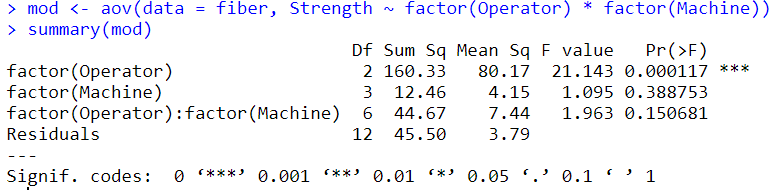
\includegraphics{13.3a.PNG}
\\From the ANOVA table, we see that the Operator factor is statistically significant at the 0.05 confidence level. On the other hand the Machine factor and the interaction are not statistically significant at the 0.05 confidence level.
\\
\\b) Variance estimates:
\\$\hat{\sigma}^2 = MSE = 3.79$
\\$\hat{\sigma_{\tau\beta}}^2 = \frac{MSAB - MSE}{n} = \frac{7.44 - 3.79}{2} = 1.83$
\\$\hat{\sigma_{\beta}}^2 = \frac{MSB - MSAB}{an} = \frac{4.15 - 7.44}{3(2)} = -0.55 < 0 \Rightarrow 0$
\\$\hat{\sigma_{\tau}}^2 = \frac{MSA - MSAB}{bn} = \frac{80.17 - 7.44}{4(2)} = 9.09$

\section*{13.7}
a) Using a mixed model is appropriate.
\\
\\b) 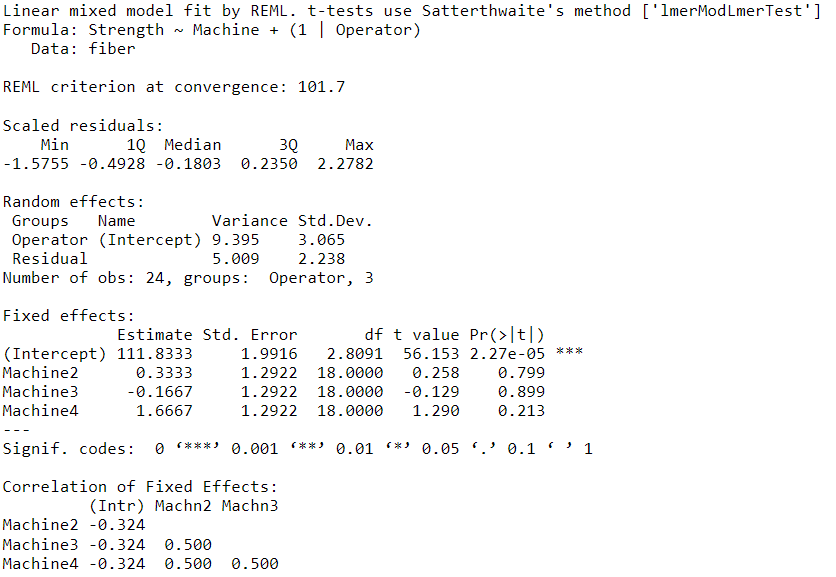
\includegraphics{13.7.PNG}

\section*{13.15}
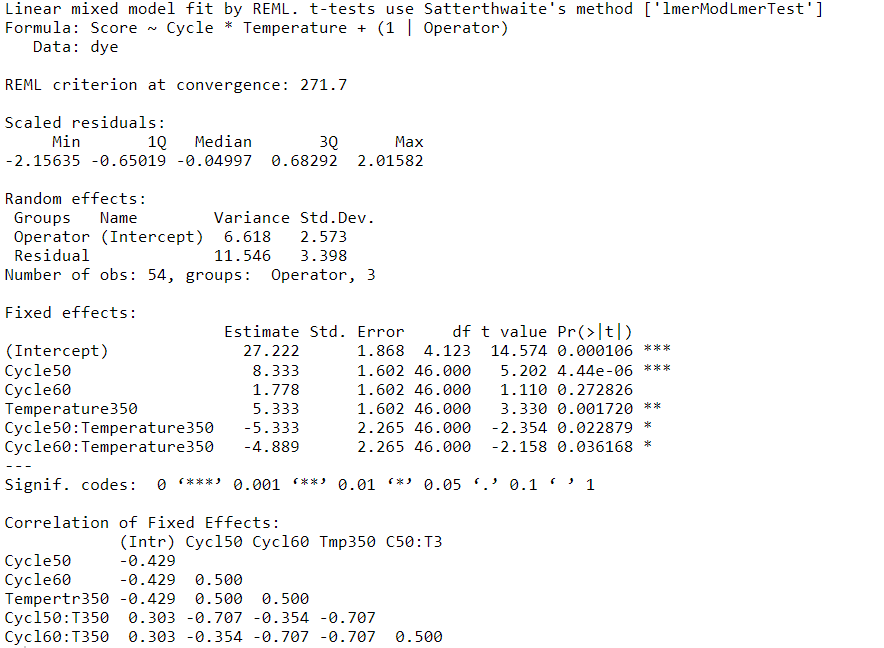
\includegraphics{13.15.PNG}
\\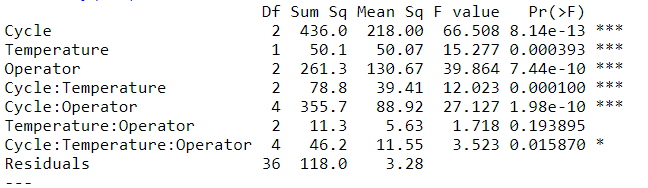
\includegraphics{13.15aov.PNG}
\\b) Variance estimates:
\\$\hat{\sigma}^2 = MSE = 3.28$
\\$\hat{\sigma_{\tau\beta\gamma}}^2 = \frac{MSABC - MSE}{n} = \frac{11.55 - 3.28}{3} = 2.76$
\\$\hat{\sigma_{\tau\beta}}^2 = \frac{MSAB - MSE}{cn} = \frac{88.92 - 3.28}{2(3)} = 14.27$
\\$\hat{\sigma_{\beta\gamma}}^2 = \frac{MSBC - MSE}{an} = \frac{5.63 - 3.28}{3(3)} = 0.26$
\\$\hat{\sigma_{\beta}}^2 = \frac{MSB - MSE}{acn} = \frac{130.67 - 3.28}{3(2)(3)} = 7.08$

\section*{13.16}
Source:
\\A: $DF = a - 1$: $E(MS) = \sigma^2 + c\sigma_{\tau\beta}^2 + bc\sigma_{\tau}^2$
\\B: $DF = b - 1$: $E(MS) = \sigma^2 + c\sigma_{\tau\beta}^2 + a\sigma_{\beta\gamma}^2 + ac\sigma_{\beta}^2$
\\C: $DF = c - 1$: $E(MS) = \sigma^2 + a\sigma_{\beta\gamma}^2 + ab\sigma_{\gamma}^2$
\\AB: $DF = (a - 1)(b - 1)$: $E(MS) = \sigma^2 + c\sigma_{\tau\beta}^2$
\\BC: $DF = (b - 1)(c - 1)$: $E(MS) = \sigma^2 + a\sigma_{\beta\gamma}^2$
\\Error $ = (AC + ABC)$: $DF = b(a - 1)(c - 1)$ : $E(MS) = \sigma^2$
\\Total $DF = abc - 1$

\section*{13.17}
We know that $\sum_{i = 1}^a (\tau\beta)_{ij} = 0$
\\Therefore its variance is 0 because it is constant.
\\$$\Rightarrow \sum_{i = 1}^a V(\tau\beta)_{ij} + \frac{2a!}{2!(a-2)!}Cov[(\tau\beta)_{ij}, (\tau\beta)_{i'j}] = 0$$
\\$$\Rightarrow a(\frac{a - 1}{a}) \sigma_{\tau\beta}^2 + \frac{2a!}{2!(a-2)!} Cov[(\tau\beta)_{ij}, (\tau\beta)_{i'j}]$$
$$\Rightarrow (a-1)\sigma_{\tau\beta}^2 + a(a-1)Cov[(\tau\beta)_{ij}, (\tau\beta)_{i'j}] = 0$$
$$\Rightarrow Cov[(\tau\beta)_{ij}, (\tau\beta)_{i'j}] = -\frac{\sigma_{\tau\beta}^2}{a}$$

\section*{13.22}
$$\frac{f_EMSE}{\chi_{\alpha/2.f_E}^2} \leq \sigma^2 \leq \frac{f_EMSE}{\chi_{1-\alpha/2.f_E}^2}$$
\\From Problem 13.3, we have:
\\$MSE = 3.79$
$$1.95 \leq \sigma^2 \leq 10.34$$
\\
\\Satterthwaite: 
$$\frac{r\hat{\sigma_{\beta}^2}}{\chi_{\alpha/2, r}^2} \leq \hat{\sigma_{\beta}}^2 \leq \frac{r\hat{\sigma_{\beta}^2}}{\chi_{1-\alpha/2, r}^2}$$
\\Where $$r = \frac{(MSAB - MSE)^2}{\frac{MSAB^2}{(a - 1)(b - 1)} + \frac{MSE^2}{df_E}}$$

\section*{13.23}
Using Satterthwaite Method same as 13.22, and
\\$\sigma_{\beta}^2 = 7.08$
\\$r = 1.9$,
\\We get $$\frac{1.9(7.08)}{7.14} \leq \hat{\sigma_{\beta}}^2 \leq \frac{1.9(7.08)}{0.05}$$
$$\Rightarrow 1.88 \leq \hat{\sigma_{\beta}}^2 \leq 294.29$$

\section*{13.26}
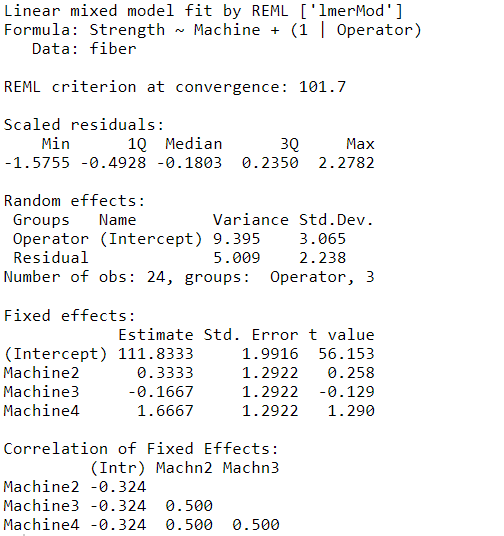
\includegraphics{13.26.PNG}
\end{document}